% Note: This file intended to be included in one of the two wrapper files in this directory.
% Hence, it has no document class.

\usepackage[utf8]{inputenc}
\usepackage{minted}
\usepackage{listings}
\usepackage{graphicx}
\usepackage{xcolor}
\usepackage{adjustbox}


\usetheme{Madrid}
\useinnertheme{circles}
\definecolor{ssgreen}{HTML}{669B41}
\usecolortheme[named=ssgreen]{structure}

%Change link colors, except for navigation links...
\definecolor{links}{HTML}{2A1B81}
\hypersetup{colorlinks,linkcolor=,urlcolor=links}
%And, except for footer links
\addtobeamertemplate{footline}{\hypersetup{allcolors=.}}{}

\setbeamertemplate{navigation symbols}{}
\setlength{\columnseprule}{0.4pt}

\AtBeginEnvironment{frame}{\setcounter{footnote}{0}}

\title[Kubernetes]{Introduction to Kubernetes}
\author[Ed MacDonald]{Ed MacDonald}
\institute{DevIgnition}
\date{November 2024}

\titlegraphic{ \includegraphics[width=2cm]{logo} }

\begin{document}
    \frame{\titlepage}

    \begin{frame}
        \frametitle{Solution Street}
        \begin{columns}
            \begin{column}{0.75\textwidth}
                \textbf{Ed MacDonald} - emacdonald@solutionstreet.com

                \vspace{1em}

                ~~ We are run by software engineers!

                ~~~~ Mostly commercial clients

                ~~~~~~ Work with the best engineers

                ~~~~~~~~ All tech stacks!

                ~~~~~~~~~~ HQ in Herndon….We are Hiring!

                \vspace{1em}

                \textbf{Find me after to learn about us}
            \end{column}
            \begin{column}{0.25\textwidth}
                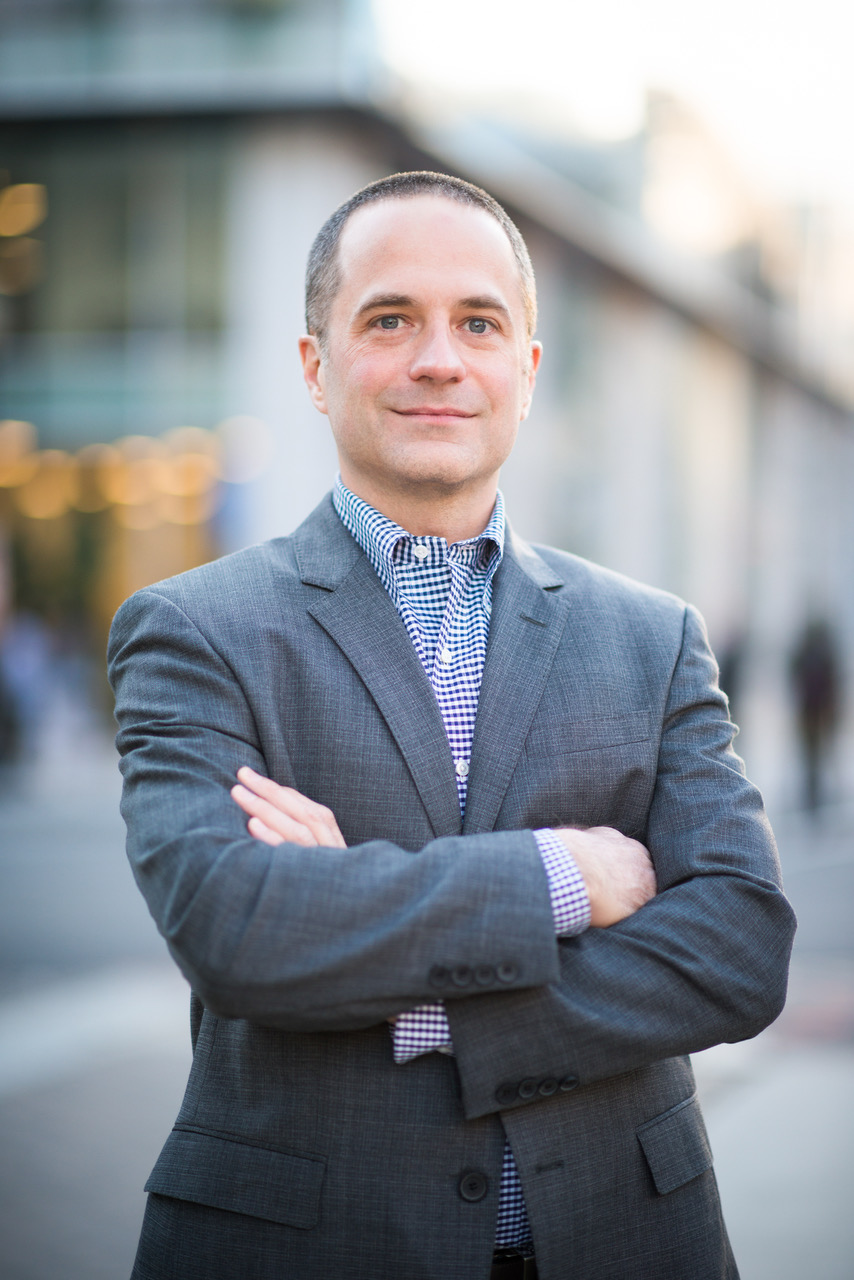
\includegraphics[width=\textwidth,height=0.85\textheight,keepaspectratio]{graphics/Headshot}
            \end{column}
        \end{columns}
    \end{frame}

    \begin{frame}
        \frametitle{What is Kubernetes?}
        \begin{itemize}
            \item{A Container Orchestration Framework.}\pause
            \item{Converges to the state you tell it to.}\pause
            \item{Very well suited for Applications that scale horizontally (stateless).}\pause
            \item{But can also accommodate portions of your infrastructure that do not scale horizontally (stateful). Don't let people tell you otherwise.}
        \end{itemize}
    \end{frame}

    \begin{frame}
        \frametitle{How do you use it?}
        \begin{itemize}
            \item{Package your Application components as Containers.}\pause
            \item{Run the Containers on Kubernetes Pods.}\pause
            \item{Let Kubernetes manage the Pods for you!}
        \end{itemize}
    \end{frame}

    \begin{frame}
        \frametitle{Why go through the hassle? (It can be a hassle)}
        Kubernetes can manage resources for you by:\pause
        \begin{itemize}
            \item{Changing the number of running Pods to meet traffic demands.}\pause
            \item{Adjusting compute resources to meet compute demands.}\pause
            \item{Replacing unresponsive Pods with new ones.}
        \end{itemize}
    \end{frame}

    \begin{frame}
        \frametitle{When can you benefit from horizontal scaling?}
        \begin{itemize}
            \uncover<1->{\item{Your app consists only of stateless components.}}
            \begin{itemize}
                \uncover<2->{\item{For example: An app that converts uploaded Word documents to PDF documents.}}
            \end{itemize}
            \uncover<3->{\item{Your app has stateless and stateful components, but the stateful components are not the bottleneck.}}
            \begin{itemize}
                \uncover<4->{\item{Consider SETI@home\footnotemark -- They farmed out intensive computations to a network of PCs, each of which presumably sent back a result that was inserted into their RDBMS.}}
            \end{itemize}
            \uncover<5->{\item{You can find a way to scale your stateful components enough that they are no longer the bottleneck.}}
            \begin{itemize}
                \uncover<6->{\item{For example: An RDBMS in a read heavy application can scale read-only replicas horizontally and distribute reads (SELECTs) among them.}}
                \uncover<7->{\item{Or in a write heavy application, perhaps the primary entity can be sharded and distributed among multiple RDBMS instances.}}
            \end{itemize}
        \end{itemize}
        \footnotetext[1]<4->{\href{https://en.wikipedia.org/wiki/SETI@home}{https://en.wikipedia.org/wiki/SETI@home}}
    \end{frame}

    \begin{frame}
        \begin{center}
            \Huge High Level Deployment Walkthrough
        \end{center}
    \end{frame}

    \begin{frame}<handout:0>
        \only<1>{\frametitle{Deploying An App: Build Your App}}
        \only<2>{\frametitle{Deploying An App: Package Your App as a Container}}
        \only<3>{\frametitle{Deploying An App: Push The Container to a Repository}}
        \only<4>{\frametitle{Deploying An App: Deploy Pods to a Kubernetes Cluster}}
        \only<5>{\frametitle{Deploying An App: Pods Pull Your Container}}

        \only<1>{\includegraphics[width=\textwidth,height=0.85\textheight,keepaspectratio]{graphics/deploy-00-app.eps}}
        \only<2>{\includegraphics[width=\textwidth,height=0.85\textheight,keepaspectratio]{graphics/deploy-01-appContainerized.eps}}
        \only<3>{\includegraphics[width=\textwidth,height=0.85\textheight,keepaspectratio]{graphics/deploy-02-containerToRepo.eps}}
        \only<4>{\includegraphics[width=\textwidth,height=0.85\textheight,keepaspectratio]{graphics/deploy-03-emptyPods.eps}}
        \only<5>{\includegraphics[width=\textwidth,height=0.85\textheight,keepaspectratio]{graphics/deploy-04-podsWithContainers.eps}}
    \end{frame}

    \begin{frame}<beamer:0>
        \frametitle{Deploying An App}
        \includegraphics[width=\textwidth,height=0.85\textheight,keepaspectratio]{graphics/deploy-04-podsWithContainers.eps}
    \end{frame}

    \begin{frame}
        \begin{center}
            \Huge Simple, right? Now let's get into the weeds.
        \end{center}
    \end{frame}

    \begin{frame}
        \frametitle{Tools}
        \begin{itemize}
            \uncover<1->{\item docker\footnotemark[1]}
            \begin{itemize}
                \uncover<2->{\item How we package our applications and put them in a place where k8s can find them.}
            \end{itemize}
            \uncover<3->{\item minikube\footnotemark[2]}
            \begin{itemize}
                \uncover<4->{\item Our very own k8s cluster on our laptop (development use only!).}
            \end{itemize}
            \uncover<5->{\item helm\footnotemark[3]}
            \begin{itemize}
                \uncover<6->{\item How we package and rollout k8s manifests.}
            \end{itemize}
            \uncover<7->{\item kubectl\footnotemark[4]}
            \begin{itemize}
                \uncover<8->{\item How we Create, Read, Update, and Delete k8s resources (when helm would be overkill).}
                \uncover<9->{\item Very thin wrapper around k8s API.}
            \end{itemize}
        \end{itemize}
        \footnotetext[1]<1->{\href{https://www.docker.com/get-started}{https://www.docker.com/get-started}}
        \footnotetext[2]<3->{\href{https://kubernetes.io/docs/tasks/tools/install-minikube}{https://kubernetes.io/docs/tasks/tools/install-minikube}}
        \footnotetext[3]<5->{\href{https://helm.sh}{https://helm.sh}}
        \footnotetext[4]<7->{\href{https://kubernetes.io/docs/tasks/tools/install-kubectl}{https://kubernetes.io/docs/tasks/tools/install-kubectl}}
    \end{frame}

    \begin{frame}
        \frametitle{Kubernetes Nodes}
        \begin{itemize}
            \uncover<1->{\item The (virtual) machines that make up the Kubernetes cluster.}
            \uncover<2->{\item Kubernetes schedules Pods to run on these Nodes.}
            \uncover<3->{\item Managed Kubernetes services\footnotemark[1] can change the number of Nodes to increase/decrease compute resources.}
        \end{itemize}
        \footnotetext[1]<3->{\href{https://aws.amazon.com/eks/}{EKS}, \href{https://azure.microsoft.com/en-us/products/kubernetes-service}{AKS}, \href{https://cloud.google.com/kubernetes-engine}{GKE}}
    \end{frame}

% https://www.patrickbaylis.com/posts/2018-10-11-beamer-resizing/
    \begin{frame}
        \frametitle{Kubernetes Nodes}
        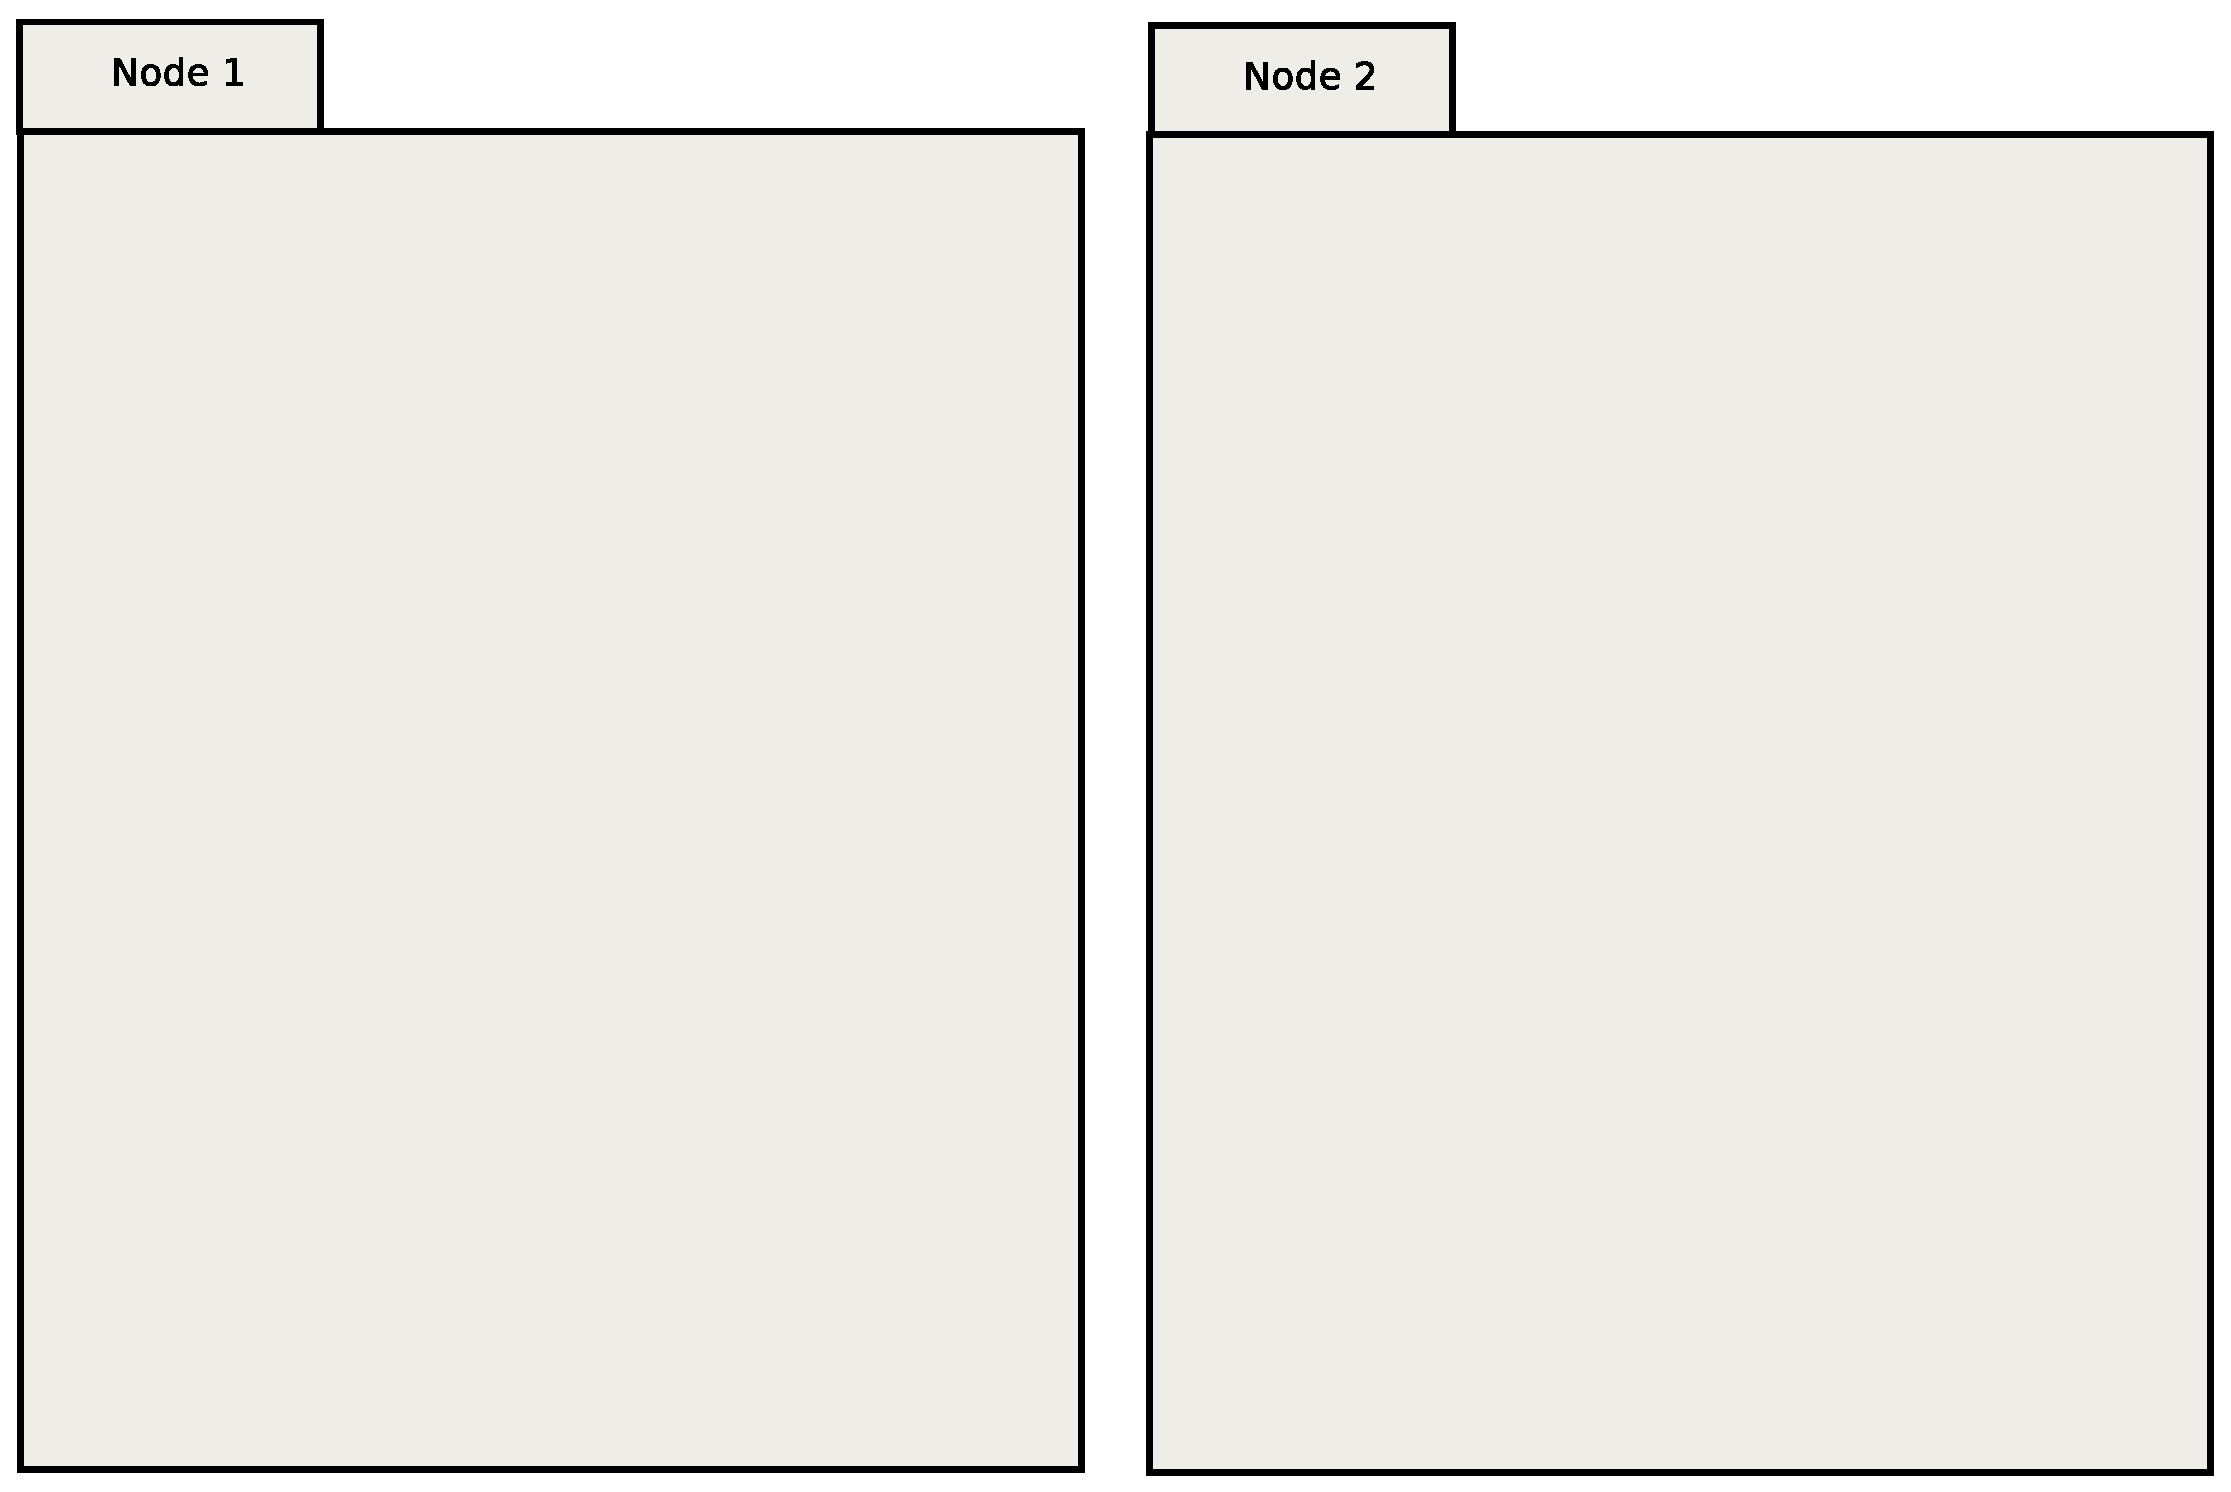
\includegraphics[width=\textwidth,height=0.85\textheight,keepaspectratio]{graphics/00-nodes.eps}
    \end{frame}

    \begin{frame}
        \frametitle{Manifest Types - K8s Building Blocks}
        \includegraphics[width=\textwidth,height=0.85\textheight,keepaspectratio]{graphics/manifest-types.eps}
    \end{frame}

    \begin{frame}
        \frametitle{Pods}
        Pods (not Containers!) are the fundamental building blocks of a Kubernetes Application\pause
        \begin{itemize}
            \item A Pod is a group of one or more Containers that work closely together on a specific task.\pause
            \item Pods manage Volumes for their Containers.\pause
            \item Pods specify health check endpoints for their Containers.\pause
            \item Kubernetes software is deployed as Pods on the cluster!
        \end{itemize}
    \end{frame}

    \begin{frame}
        \frametitle{ReplicaSets (Stateless Pod Controllers)}
        \begin{itemize}
            \item Pods come and go.\pause
            \begin{itemize}
                \item Replaced if unresponsive.\pause
                \item Can be deleted on one Node and added on another (moved).\pause
                \item \textbf{You cannot prevent either of these things from happening.}\pause
            \end{itemize}
            \item With ReplicaSets\pause
            \begin{itemize}
                \item Volumes don't follow Pods.\pause
                \item Hostnames don't follow Pods.
            \end{itemize}
        \end{itemize}
    \end{frame}

%    \begin{frame}
%        \frametitle{Controllers}
%        \begin{itemize}
%            \item Don't create Pods directly.
%            \item Instead, create a Controller that manages the Pods for you.
%        \end{itemize}
%    \end{frame}
%
%    \begin{frame}
%        \frametitle{Controllers: ReplicaSets}
%        \begin{itemize}
%            \item State how many Pods you want.\pause
%            \item Pods are treated as if they were stateless.\pause
%            \item From Application's point of view, Pods in a ReplicaSet are indistinguishable.
%        \end{itemize}
%    \end{frame}

    \begin{frame}
        \frametitle{Deployment (Controller)}
        \begin{itemize}
            \item ReplicaSets with more features.\pause
            \item I'm not going to use those features.\pause
            \item But I use Deployments because helm produces them for skeleton helm projects.
        \end{itemize}
    \end{frame}

    \begin{frame}
        \frametitle{Serivce (Load Balancer)}
        \begin{itemize}
            \item Load Balancers have an internal cluster IP address.\pause
            \item They can also have an external IP address.\pause
            \item They distribute requests sent to either IP address to all Pods targeted by their ``selector".
        \end{itemize}
    \end{frame}

    \begin{frame}
        \frametitle{The Sample App}
        I wrote an Application that does nothing other than suggest a random Subreddit.\pause
        \begin{itemize}
            \item Stateless.\pause
            \item Selects at random from a list of 280 Subreddits.\pause
            \item The list never changes.\pause
            \item It doesn't need to store anything anywhere.
        \end{itemize}
    \end{frame}

    \begin{frame}
        \frametitle{Load Balancers}
        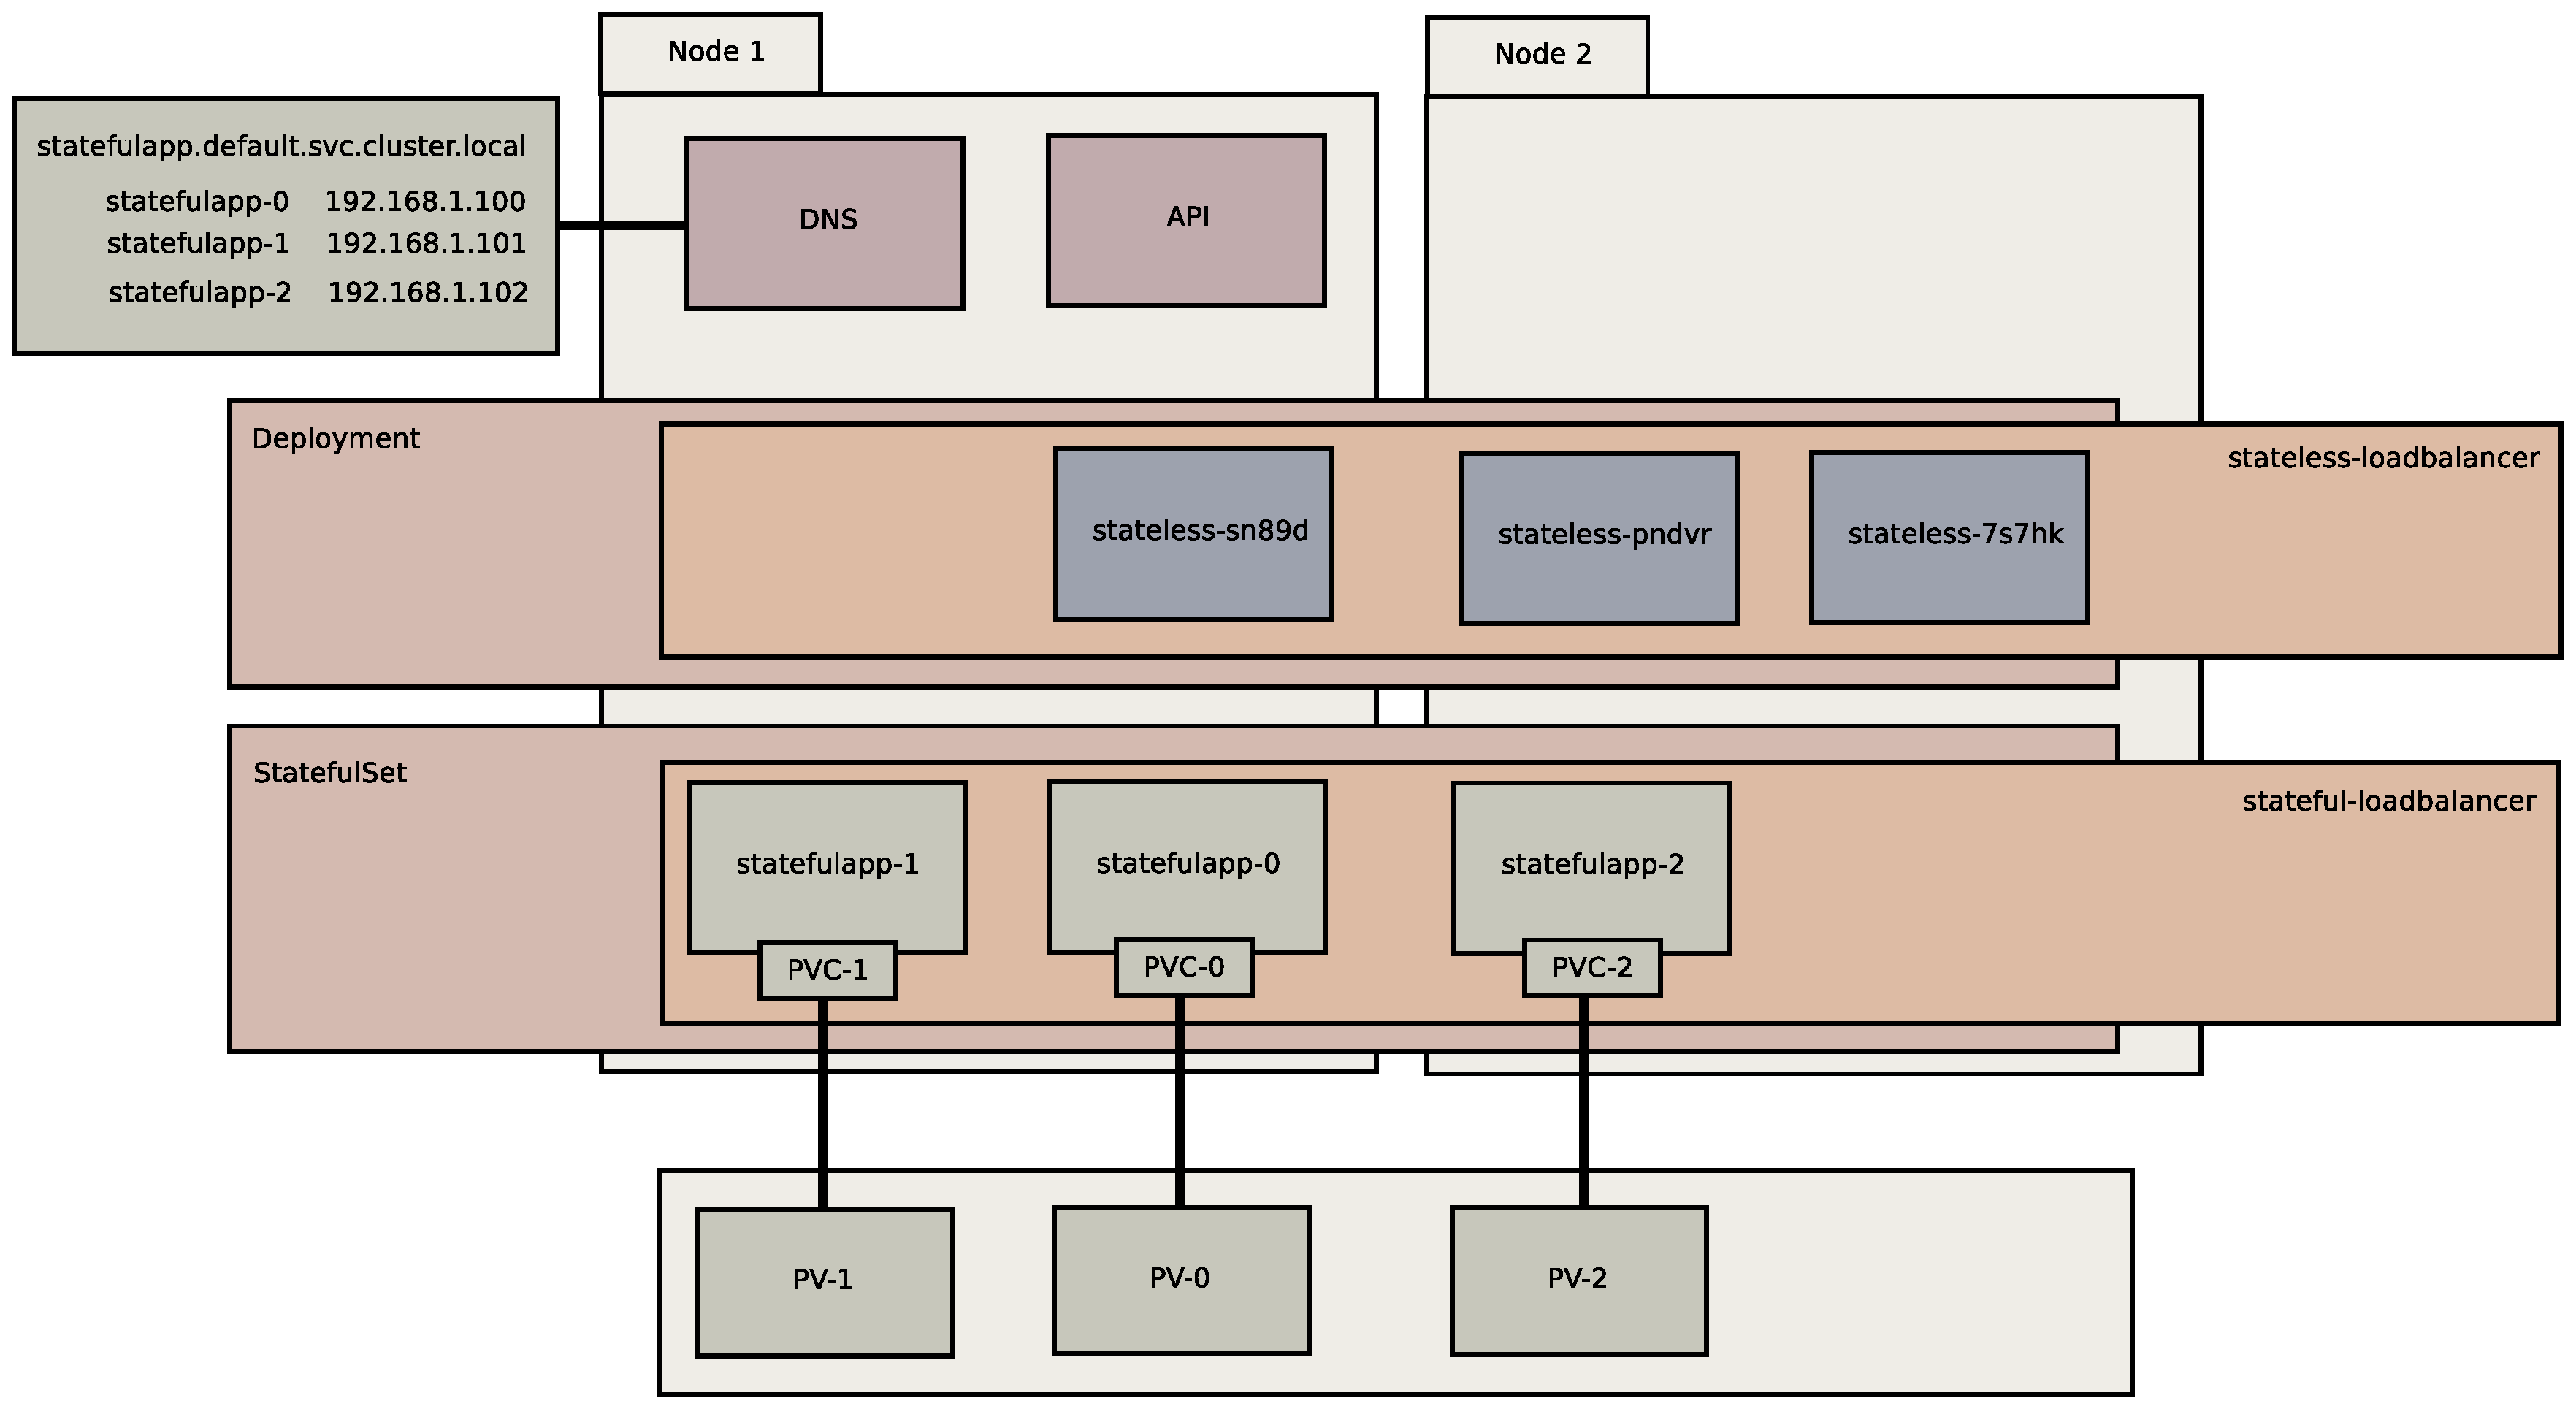
\includegraphics[width=\textwidth,height=0.85\textheight,keepaspectratio]{graphics/08-loadBalancer.eps}
    \end{frame}

    \begin{frame}
        \frametitle{Demo}
        \begin{center}
            \Huge So, let's see this in action!
        \end{center}
    \end{frame}

    \begin{frame}
        \frametitle{Overview}
        First, let's talk about the steps we're going to take:
        \begin{itemize}
            \item Start our Kubernetes environment (minikube).\pause
            \item Configure our docker cli to talk to minikube's docker host.\pause
            \item Build our two sample Applications, package them as docker Containers, and push the images.\pause
            \item Run helm to deploy our Kubernetes components.\pause
            \item Proxy local ports to connect to our load balancing services.
        \end{itemize}
    \end{frame}

    \begin{frame}
        \frametitle{Demo Architecture}
        \includegraphics[width=\textwidth,height=0.85\textheight,keepaspectratio]{graphics/simplifiedModel-00.eps}
    \end{frame}

    \begin{frame}
        \begin{center}
            \Huge Is there enough time to go deeper?\\
            If so, let's dig into some code.
        \end{center}
    \end{frame}

    \begin{frame}
        \frametitle{Other Resources}
        Peripheral tools I used -- some of which warrant their own presentation
        \begin{itemize}
            \item \LaTeX: \href{https://www.latex-project.org}{https://www.latex-project.org}
            \item Beamer: \href{https://ctan.org/pkg/beamer}{https://ctan.org/pkg/beamer}
            \item Kotlin: \href{https://kotlinlang.org}{https://kotlinlang.org}
            \item Spring Boot: \href{https://spring.io/projects/spring-boot}{https://spring.io/projects/spring-boot}
            \item Gradle: \href{https://gradle.org}{https://gradle.org}
            \item Dia: \href{http://dia-installer.de}{http://dia-installer.de}
        \end{itemize}
        \smallskip
        Where I got my Subreddit data
        \begin{itemize}
            \item Bulk Reddit data: \href{http://files.pushshift.io/reddit/subreddits}{http://files.pushshift.io/reddit/subreddits}
        \end{itemize}
        Finally, \textbf{\textit{this}} demo
        \begin{itemize}
            \item \href{https://github.com/emacdona/k8sdemo}{https://github.com/emacdona/k8sdemo}
        \end{itemize}
    \end{frame}

    \begin{frame}
        \frametitle{A Note on Capitalization}
        I agonized over which words to capitalize.
        \begin{itemize}
            \item{I capitalized important concepts in the Kubernetes domain:}
            \begin{itemize}
                \item{Any Kubernetes component: Deployment, Pod, ReplicaSet, StatefulSet, ...}
                \item{Application, Container, Kubernetes, Node, Volume}
            \end{itemize}

            \item{But some didn't quite make the cut:}
            \begin{itemize}
                \item{cluster, component}
            \end{itemize}

            \item{I could not bring myself to capitalize things that I type at the command prompt:}
            \begin{itemize}
                \item{docker, helm, kubectl, minikube}
            \end{itemize}
        \end{itemize}
    \end{frame}

    \begin{frame}
        \begin{center}
            \Huge Questions?
        \end{center}
    \end{frame}

\end{document}
